%! TEX root = 2_sistem_rangka_kaku.tex
% the main TeX file which is intended to compile, :VimtexReload after adjustment
   % this file should be included in the main file
% :h vimtex-tex-root
\documentclass[../modul_skb.tex]{subfiles}
%ensure the class of docs
\begin{document}

\section{Sistem Struktur Rangka Kaku}%
\label{sec:Sistem Struktur Rangka Kaku}

Pada bangunan tinggi gaya-gaya yang bekerja dari luar bangunan sangat mempengaruhi perancang dalam memilih sistem struktur dan kinerja yang dihasilkan. Adapun gaya yang dominant berpengaruh adalah gaya tekan angin dan gaya lateral. Gaya tekan angin yang menghasilkan eksentrisitas dimana menimbulkan gaya torsi pada bangunan, membuat kecenderungan bangunan memerlukan sistem struktur yang dapat menahan gaya torsi dan puntir untuk mencegah terjadinya buckling. Selain itu gaya horizontal, gaya lateral yang bekerja mengenai sebuah bangunan juga perlu direspon dalam suatu sistem struktur. Maka dari itu diperlukan sebuah sistem struktur yang mampu menahan beban gaya tekan angin dan gaya lateral. Struktur rigid frame merupakan sistem struktur yang perlu dianalisa lebih lanjut apakah dapat memenuhi kedua permasalahan tersebut

Rangka kaku dan inti (rigid frame and core) Merupakan rangka hybrid dimana adanya penggabungan sistem struktur rangka kaku (rigid frame) an sistem struktur inti (core). Rangka kaku bereaksi terhadap beban lateral, terutama melalui lentur balok dan kolom. Perilaku demikian berakibat ayunan (drift) lateral yang besar pada bangunan dengan ketinggian tertentu. Akan tetapi, apabila dilengkapi dengan struktur inti, ketahanan lateral bangunan akan sangat meningkat karena interaksi inti dan rangka. Sistem inti ini memuat sistem-sistem mekanis dan transportasi vertikal. Untuk lebih memahami tentang sistem ini, kita akan membahas karakteristik dari masingmasing sistem struktur.

\subsection{Sistem Core (Inti Bangunan)}%
\label{sub:Sistem Core (Inti Bangunan)}


Struktur \textbf{core} wall yang bisa dijumpai dalam aplikasi konstruksi bangunan tinggi dewasa ini ada bermacam-macam. Antara lain adalah bentuk $\square$,$\triangle$,$\circ$ atau \textbf{core} wall dua cell dengan pengaku di tengahnya berbentuk $\boxminus$. Dari masing-masing bentuk \textbf{core} wall ini, mempunyai karakteristik yang berbeda-beda dalam memberikan fleksibilitas dan efektivitas pada struktur bangunan. Bangunan tinggi yang mempunyai struktur \textbf{core} wall, dibuat dengan salah satu pertimbangan adalah fleksibilitas untuk pengaturan posisi (tata letak) yang akan memberikan penghematan dan efisiensi maksimum pada bangunan secara keseluruhan. Pada sistim \textbf{core} (inti) sebagai pengaku bangunan secara keseluruhan, dimana gayagaya lateral yang bekerja disalurkan oleh balok-balok menuju ke \textbf{core}/inti sebagai elemen struktur utama. \textbf{Core} sebagai inti pengaku pendukung utama struktur bangunan, dengan material dari :

\begin{itemize}
	\item Core beton (shear wall atau bearing wall)
	\item Core dari struktur baja (tube)
\end{itemize}


Posisi perletakan \textit{sistim core} pada bangunan tergantung pada titik pusat keseimbangannya, dimana perletakkannya mempunyai beberapa varian, seperti :

\begin{itemize}
	\item Sentral core, dimana core (inti) terletak pada titik pusat massa bangunan.
	\item Core pada tepi bangunan, berfungsi sebagai penahan gaya lateral secara langsung \textit{``lateral core"}.
	\item Bangunan dengan 2 (dua) core, dimana perletakan core pada kedua sisi bangunan.
	\item Bangunan dengan core tersebar, dengan perletakan core tersebar pada seluruh bidang bangunan dan berada pada titik berat bangunan.
	\item Core dengan shear wall, yang berguna untuk kekakuan. Dimana core dipadu dengan shear wall (dinding geser), sedang shear wall berperan sebagai penahan gaya geser daripada gaya horizontal.
	\item Core dengan rangka kaku (baja), merupakan penggabungan core dengan rangka kaku sehingga menjadi satu kesatuan yang kaku dan stabil.
\end{itemize}

Dan yang paling penting adalah bahwa sistem struktur core wall ini didesain untuk dapat manahan gaya torsi yang timbul akibat tekanan angin yang eksentrisitas dan seragam pada pusat geser struktur core wall. Struktur core wall pada dasarnya adalah sistem struktur yang dibuat untuk mampu menahan gaya-gaya lateral yang timbul akibat gaya angin atau gempa yang merupakan beban dinamis. Untuk proses analisis mekanikanya, pengaruh gaya-gaya akibat beban angin dan gempa tersebut (yang merupakan beban dinamis) diperlakukan sebagai beban statis dan mengabaikan sifat dinamisnya.

\begin{figure}
	\begin{center}
		
\includegraphics[width=.82\textwidth]{core}
		% filename may not contain space but _
	\end{center}
	\caption{Struktur Core}
	\label{fig:strcore}
\end{figure}

Kondisi eksentrisitas tekanan angin tersebut secara teknis dapat terjadi antara lain adalah karena :

\tabitem Posisi struktur core wall yang ditempatkan di dalam bangunan.

Penempatan struktur core wall yang dekat kepada pusat bangunan akan memberikan eksentrisitas tekanan angin yang berkurang, yang juga akan memperkecil pengaruh gaya torsi yang terjadi. Namun secara praktis untuk membuat pengaruh gaya torsi tidak ada (nol) sama sekali dalam konstruksi bangunan di lapangan adalah mustahil, dikarenakan gaya angin yang terjadi tidak pernah seragam dan simetris. Sudut datang gaya angin itu sendiri merupakan faktor penentu sebagai komponen yang mempunyai nilai berbeda untuk setiap sudut datang yang berbeda, yang sudah tentu akan menghasilkan torsi yang berbeda pula.

Selain itu, yang pasti bentuk bangunan dan lubang-lubang pada struktur core wall juga dapat mempengaruhi nilai torsi yang timbul.

Sistem rangka kaku murni dalam perkembangannya tidak praktis untuk bangunan yang lebih tinggi dari 30 lantai. Berbagai sistem telah diterapkan dengan menggunakan dinding geser didalam rangka untuk menahan beban lateral. Dinding ini terbuat dari beton atau rangka baja. Bentuknya bisa berupa inti interior tertutup, mengelilingi ruang lift atau ruang tangga, atau bisa berupa dinding sejajar di dalam bangunan, bahkan bisa juga berupa rangka fasade vertikal.

Untuk bangunan apartement, kebutuhan jaringan akan fungsi dan utilitas cenderung tetap, tetapi untuk bangunan komersial membutuhkan fkelsibilitas dalam hal tata letak yang memerlukan ruang terbuka yang cukup lebar dengan dinding partisi yang dapat dipindahpindah. Untuk yang menggunakan sistem struktur inti, inti dapat dipergunakan untuk menempatkan sistem transportasi vertikal, tangga, wc, shaft, dan jaringan utilitas lainnya sehingga kadang bangunan mempunyai inti yang lebih dari satu.

Beberapa bangunan tinggi menggunakan inti dan rangka. Dari segi perilaku denah ini diterapkan untuk memuaskan sistem plat datar atau dinding rangka geser bersama belt trusses. Inti dapat terbuat dari beton , baja atau konbinasi antara betoin dan baja. Keuntungan inti baja, dalam perakitan lebih cepat karena pabrikasi. Sedangkan inti dari beton menghasilkan ruang yang sekaligus memikul beban. Juga dapat dipakai untuk perlindungan saat kebakaran.

Bentuk denah yang bermcam-macam menungkinkan perletakan sejumlah inti bangunan. Sistem inti ini dikaitkan dengan bentuk bangunan yang diatur menurut letaknya, seperti:

\begin{itemize}
	\item Letak inti :
	      \begin{itemize}
		      \item inti fasade eksterior (diluar)
		      \item inti interior : inti fasade (sekeliling)
		      \item inti didalam bangunan
	      \end{itemize}
	\item Jumlah inti :
	      \begin{itemize}
		      \item inti tunggal
		      \item inti terpisah
		      \item inti banyak
	      \end{itemize}
	\item Bentuk inti :
	      \begin{itemize}
		      \item inti tertutup : bujur sangkar, persegi panjang, bulat, segitiga
		      \item inti bentuk terbuka : bentuk X, I dan [
		      \item Bentuk inti disesuaikan dengan bentuk bangunan
	      \end{itemize}
	\item Susunan inti :
	      \begin{itemize}
		      \item Simetris
		      \item Asimetris
	      \end{itemize}
\end{itemize}

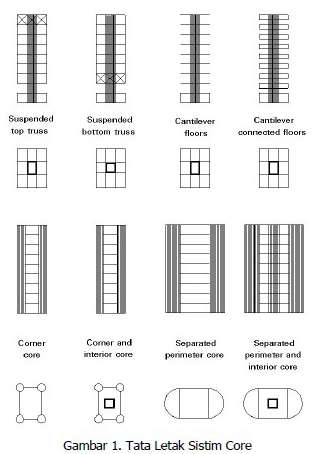
\includegraphics[width=.82\textwidth]{../figures/tata_letak_core.jpeg}

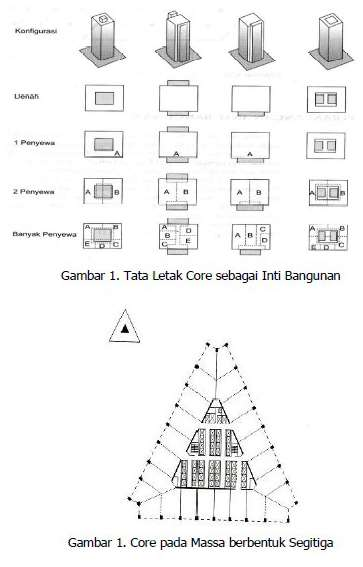
\includegraphics[width=.82\textwidth]{../figures/core_segitiga.jpeg}

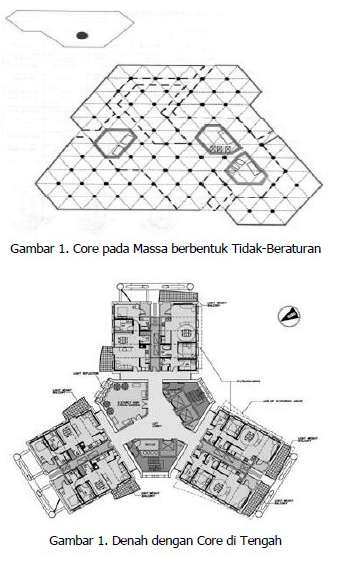
\includegraphics[width=.82\textwidth]{../figures/core_tdk_beraturan.jpeg}

\subsection{Sistem Rangka Kaku (Rigid Frame}%
\label{sub:Sistem Rangka Kaku (Rigid Frame}

Bentuk struktur rangka adalah perwujudan dari pertentangan antara gaya tarik bumi dan kekokohan; dan struktur rangka yang modern adalah hasil penggunaan baja dan beton secara rasional dalam bangunan. Kerangka ini terdiri atas komposisi dari kolom-kolom dan balok-balok. Unsur vertikal, berfungsi sebagai penyalur beban dan gaya menuju tanah, sedangkan balok adalah unsur horizontal yg berfungsi sebagai pemegang dan media pembagian lentur.

Kemudian kebutuhan-kebutuhan terhadap lantai, dinding dan sebagainya untuk melengkapi kebutuhan bangunan untuk hidup manusia, dapat diletakkan dan ditempelkan pada kedua elemen rangka bangunan tersebut diatas. Jadi dapat dinyatakan disini bahwa rangka ini berfungsi sebagai struktur bangunan dan dinding-dinding atau elemen lainnya yang menempel padanya merupakan elemen yang tidak struktural. Bahan-bahan yang dapat dipakai pada struktur ini adalah kayu, baja, beton atau lain-lain bahan yang tahan terhadap gaya tarik, tekan, punter, dan lentur.

Untuk masa kini banyak digunakan baja dan beton yang mampu menahan gaya-gaya tersebut dalam skala besar. Untuk bahan pengisinya dapat dipakai bahan yang ringan atau yang tidak mempunyai daya dukung yang besar seperti susunan batu bata, dinding-dinding kayu, kaca dan lain-lain. Untuk sistem struktur semacam ini dimungkinkan didapatnya bangunan bertingkat banyak untuk memenuhi kebutuhan, bila dibandingkan dibandingkan dengan sistem kontruksi yang lain. Hanya ada kekurangannya, yaitu jarak antara kolom mempunyai batas maksimum yang relatif kecil. Jarak antar kolom yang jauh akan mempengaruhi dimensi dari balok mendatar yang akan membesar dan akan menjadi tidak
ekonomis.

Struktur rangka kaku (rigid frame) adalah struktur yang terdiri atas elemen-elemen linear, seperti kolom dan balok yang ujung ujungnya dihubungkan dengan joints (titik hubung) yang bersifat kaku atau rigid, bedakan dengan struktur pos-and-beam yang titik hubungnya bersifat sendi atau roll. Aksi lateral pada rangka menimbulkan lentur, gaya geser, dan gaya aksial pada semua elemen (balok dan kolom). Momen lentur akibat lateral akan mencapai maksimum pada penampang dekat titik hubung. Sehingga ukuran elemen struktur didekat titik hubung harus dibuat lebih besar atau diperkuat. Efek beban lateral yang bekerja pada struktur rangka kaku gedung bertingkat banyak, dimana semakin tinggi gedung semakin besar momen dan gaya-gaya pada setiap elemen. Apabila gaya yang bekerja sudah sedemikian besar, maka diperlukan kontribusi struktur lain, seperti bracing, sistim core ataupun dinding geser.

Distribusi gaya pada struktur rangka pada gedung tingkat banyak, apabila gedung mengalami gaya lateral maka akan terjadi kolom yang mengalami gaya tarik dan mengalami gaya tekan. Struktur rangka (rigid frame) merupakan struktur yang terdiri atas elemenelemen linear, umumnya balok dan kolom, yang ujungujungnya dihubungkan dengan joints (titik hubung) yang dapat mencegah rotasi relatif diantara elemen struktur yang dihubungkannya. Dan untuk memahami perilaku struktur rangka sederhana adalah dengan membandingkan perilakunya terhadap beban dengan struktur post-andbeam. Kerangka terdiri atas komposisi kolom-kolom dan balokbalok. Unsur vertikal berfungsi sebagai penyalur beban dan gayagaya menuju tanah, sedangkan balok adalah unsur horizontal sebagai pemegang dan media pembagi beban dan gaya menuju kolom. Efek turunnya tumpuan (support settlement) pada struktur rangka, karena adanya perbedaan penurunan tumpuan.

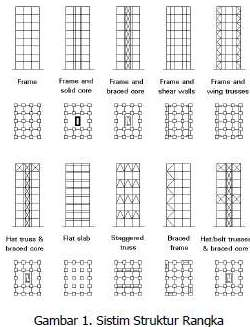
\includegraphics[width=.9\textwidth]{../figures/str_rangka_cth.jpeg}


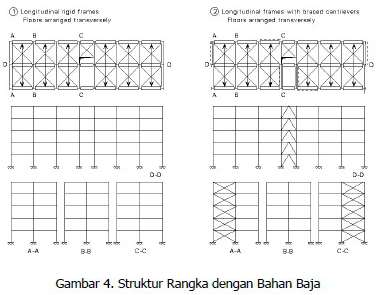
\includegraphics[width=.86\textwidth]{../figures/rangka_baja.jpeg}


Sistem Bangunan Dinding Rangka Geser (Frame- Shear Wall Building System) Sistem rangka kaku murni tidak praktis untuk bangunan yang lebih tinggi dari 30 lantai, berbagai sistem telah dicoba untuk menggunakan dinding geser di dalam rangka untuk menahan beban lateral. Dinding geser terbuat dari beton atau rangka baja, dapat berupa inti interior tertutup, mengelilingi ruang lift atau ruang tangga, atau bisa juga berupa dinding sejajar dalam bangunan. Beberapa denah bangunan tinggi tipikal yang menggunakan inti dan rangka diperlihatkan.

\begin{figure}
	\begin{center}
		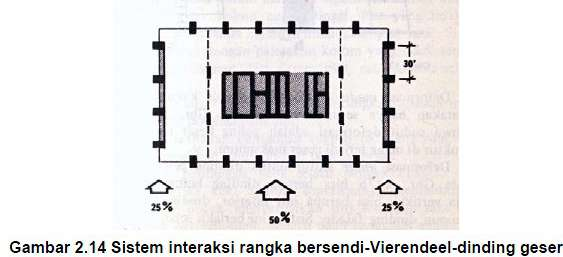
\includegraphics[width=.82\textwidth]{../figures/shear_wall.jpeg}
		% filename may not contain space but _
	\end{center}
	\caption{Sistem Interaksi rangka bersendi-Vierendeel- dinding geser}
	\label{fig:vierendeel}
\end{figure}


\begin{figure}
	\begin{center}
		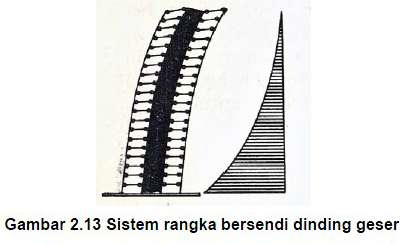
\includegraphics[width=.82\textwidth]{../figures/rangka_sendi.jpeg}
		% filename may not contain space but _
	\end{center}
	\caption{Sistem Rangka Bersendi Dinding geser}
	\label{fig:sendi}
\end{figure}


\subsubsection{Sistem rangka bersendi dinding geser}

Karena balok rangka diberi persendian, maka rangka ini hanya dapat memikul beban gravitasi. Dinding geser akan memikul semua beban lateral. Gambar~\ref{fig:sendi} Sistem rangka bersendi dinding geser

\subsubsection{Sistem interaksi rangka bersendi-Vierendeel-dinding geser}%

Gaya – gaya lateral dipikul oleh sistem dinding geser dan rangka kayu. 10 Pada contoh gambar~\ref{fig:vierendeel }, kedua dinding fasade pada arah pendek bangunan akan memikul separuh jumlah gaya angin, dan inti akan memikul separuh sisanya. Rangka fasade memanjang hanya memikul gaya gravitasi.

\subsubsection{Interaksi rangka kaku-dinding geser}%

Di atas 500 kaki, penggunaan hanya dinding geser untuk menahan beban lateral menjadi tidak praktis. Agar cukup kuat, inti harus sedemikian besar sehingga tidak sesuai lagi dengan fungsinya sebagai wadah transportasi vertikal dan distributor energi. Lebih jauh lagi, lendutan yang terjadi akan demikian besarnya sehingga menyebabkan keretakan partisi atau jendela, bahkan dapat menimbulkan reaksi psikologis pada penghuni bangunan. Kekakuan lateral sangat diperbaiki dengan menggunakan tidak hanya sistem dinding geser, tetapi juga rangka kaku untuk menahan gaya – gaya lateral. Defleksi total sistem dinding geser dan rangka kaku diperoleh dengan cara membuat superimpose mode individual dari deformasi. Dari penjabaran kedua sistem struktur tersebut, rigid frame and core adalah sistem struktur yang terdiri atas penggabungan secara horizontal sistem elemen-elemen linear, seperti kolom dan balok yang ujung ujungnya dihubungkan dengan joints (titik hubung) yang bersifat kaku atau rigid, bedakan dengan struktur pos-and-beam yang titik hubungnya bersifat sendi atau roll dengan sebuah struktur massif di dalamnya yang menerus secara vertical. Penyatuan kedua sistem struktur ini saling menguatkan kelemahan dari masing-masing struktur. Adanya struktur inti, memperkuat bangunan dari gaya torsi yang diakibatkan oleh eksentrisitas akibat tekanan angin.

\subsubsection{Interaksi rangka kaku-dinding geser}%

Di atas 500 kaki, penggunaan hanya dinding geser untuk menahan beban lateral menjadi tidak praktis. Agar cukup kuat, inti harus sedemikian besar sehingga tidak sesuai lagi dengan fungsinya sebagai wadah transportasi vertikal dan distributor energi. Lebih jauh lagi, lendutan yang terjadi akan demikian besarnya sehingga menyebabkan keretakan partisi atau jendela, bahkan dapat menimbulkan reaksi psikologis pada penghuni bangunan. Kekakuan lateral sangat diperbaiki dengan menggunakan tidak hanya sistem dinding geser, tetapi juga rangka kaku untuk menahan gaya – gaya lateral. Defleksi total sistem dinding geser dan rangka kaku diperoleh dengan cara membuat superimpose mode individual dari deformasi. Dari penjabaran kedua sistem struktur tersebut, rigid frame and core adalah sistem struktur yang terdiri atas penggabungan secara horizontal sistem elemen-elemen linear, seperti kolom dan balok yang ujung ujungnya dihubungkan dengan joints (titik hubung) yang bersifat kaku atau rigid, bedakan dengan struktur pos-and-beam yang titik hubungnya bersifat sendi atau roll dengan sebuah struktur massif di dalamnya yang menerus secara vertical. Penyatuan kedua sistem struktur ini saling menguatkan kelemahan dari masingmasing struktur. Adanya struktur inti, memperkuat bangunan dari gaya torsi yang diakibatkan oleh eksentrisitas akibat tekanan angin.

\subsection{Stabilisasi Inti dalam Rangka}

Dalam konstruksi rangka, metode stabilisasi dan kekakuan bangunan menjadi ikut meningkat seiring dengan meningkatnya jumlah lantai. Kebanyakan menara tangga dan ruang lift mengarah pada inti bangunan agar bangunan tetap stabil dan kaku dan memepertahankannya terhadap beban angin.

Para perancang seringkali mendesain poros inti beton untuk pelayanan lift dan mekanik sebagai kolom kaku besar, yang dapat disandari oleh sebuah struktur rangka. Subsistem atap dan subsistem lantai membentuk pelat diafragma yang besar dan tidak memerlukan transfer momen ke kolom vertical sehingga balok sederhana dapat digunakan pada sambungan kolom. Sambungan sederhana juga menyambungkan diafragma horizontal ke rangka pengekang atau ke dinding beton yang memikul gaya lateral.

Sebaliknya, apabila sebuah struktur harus bebas dari rangka pengekang x atau rangka pengekang K, atau bebas dari dinding geser solid untuk mempertahankan sebuah bentuk ruang yang terbuka, maka rangka struktur tersebut dapat saja menahan baik gaya lateral maupun gaya vertical sebagai struktur rangka kaku atau rangka momen. Pada kasus ini, semua balok mentransfer gaya-gaya dan momen-momen lentur ke sambungan kolom melalui sambungan momen kaku. Rangka momen sangat memerlukan balok-balok yang lebih besar dan kolom-olom yang lebih besar, terutama pada tingkat bawah struktur tinggi. Semua elemen struktur dalam sebuah rangka momen sebenarnya merupakan balok, kolom, dan interaksi tegangan serta kerampingan kolom harus ditinjau dalam analisis dan desain dari elemen-elemen struktur tersebut.

Untuk struktur yang sangat tinggi atau struktur yang berada dalam daerah yang memiliki intensitas seismic yang tinggi, sistem penahan-beban redundan lateral campuran dapat digunakan, dimana rangka momen dirangkaikan pada sistem rangka batang, sistem dinding geser, dan atau sistem pengekang lateral poros inti. Redudansi menghasilkan jalurjalur beban dalam jumlah yang banyak pada sebuah sistem struktur, sehingga dalam batas tertentu, satu sistem bekerja sebagai cadangan bagi sistem yang lainnya dalam suatu kejadian struktur yang berbahaya. Selain itu, dengan menggunakan berbagai jenis sistem pengekang, yang masing-masing memiliki karakteristik respons dinamis dari sebuah struktur, sehingga struktur tersebut dapat diselaraskan untuk menahan resonansi dengan beban-beban gempa bumi dan beban-beban angina yang dinamis. Dan dengan elemen linear dapat lebih menahan gaya lateral karena ujung ujungnya dihubungkan dengan joints (titik hubung) yang dapat mencegah rotasi relatif diantara elemen struktur yang dihubungkannya.

Berikut adalah beberapa contoh pengolahan sistem struktur rigid frame and core pada denah :

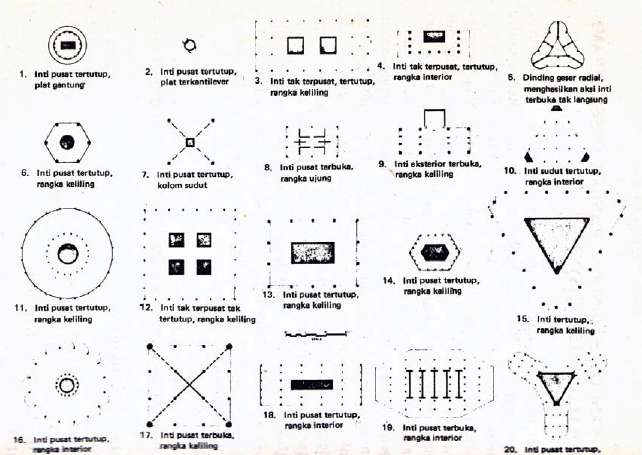
\includegraphics[width=.86\textwidth]{../figures/cth_ranka_kaku.jpeg}


\subsection{Implementasi}%
\label{sub:Implementasi}

\subsubsection{Turning Torso}%
\label{ssub:Turning Torso}

HSB Turning Torso merupakan sebuah pencakar langit di Malmö, Swedia, terletak di selat Öresund. Menara ini dirancang oleh arsitekS panyol, Santiago Calatrava dan secara resmi dibuka pada 27 Agustus 2005. Menara ini mencapai tinggi 190 meter (623 kaki) dengan 54 tingkat. Setelah selesai, menara ini menjadi bangunan tertinggi di Skandinavia, dan bangunan apartemen tertinggi kedua di Eropa, setelahTriumph-Palace setinggi 264 meter di Moskow.

\begin{itemize}
	\item \textbf{Konsep Desain}
	\item[] Desain berawal dari hasil sculpture yang di buat calatrava pada tahun 1991 yang berupa 9 buah kubus yang di tumpuk dan terpuntir sebesar 90 derajat dari bawah hingga ke puncak. Diciptakan untuk meningkatkan dan memperbesar area publik, yang didefinisikan oleh persimpangan dua jalan utama, "Turning Torso" bangunan adalah dimaksudkan untuk dilihat sebagai elemen yang berdiri bebas patung diajukan dalam Cityscape.

	\item Struktur dan konstruksi

	\item[] Bangunan tingkat tinggi sangat Rentan terhadap gaya lateral, rangka kaku dengan tambahan bracing seperti bracing diagonal atau rigid core, pada bangunan ini untuk menyeimbangi lekungan bentuknya, maka bracingnya menggunakan pilar – pilar baja yangmengelilingi tepi bangunan yang saling menyilang dibaut dengan diafragma yang kaku. Struktur tersebut akan berlaku seperti balok kotak berkantilever dalam menahan gaya – gaya lateral.
	\item[] Jendela-jendela pada bangunan ini dibuat kecil, karena dengan menggunakansistem Biering wall. jendela yang besar akan mengurangi kekuatan bangunan. Beban bangunan itu sendiri berkurang. Frame tube pada bangunan memiliki kolom – kolom yang rapat mengelilingi dan terhubung secara kaku dengan balok – balok spaderal. Perforated shelltube pada bangunan ini dibuat bergeser dan tertarik dengan bukaan dengan ritme yang teratur diikat bersamaan dengan barace. Latticed truss tube berkelilIng secara diagonal sesuai kemiringan yang rapat tanpa kolom.

	\item[]  Bangunan ini dibangun menggunakan struktur shear wall yang berupa inti bangunan ditambah dengan rangka luar. Lantai-lantai menjorok dan memutar secara individual tiap lantainya sehingga tidak mengakibatkan perubahan berarti pada lantai lainnya.
	\item[]  Rangka luar yang berbentuk segitiga terlihat seperti menggantung merupakan bagian dari struktur tower. Brancing segitiga pada bagian bawah menyalurkan gaya kembali ke core. Penyangga ke atas yang berfungsi sebagai tempat tumpuan dari bagian sudut pelat lantai.

	\item[] Sebuah rangka luar (eksoskeleton) menerus dari bawah hingga ke puncak bangunan terbuat dari baja. Rangka ini terhubung dengan kolom-kolom bangunan oleh tabung-tabung sekunder yang mengikat. Rangka luar ini memiliki fungsi menahan gaya horizontal akibat angin dan getaran.

	\item[] Core yang terbuat dari beton terletak tepat di tengah sehingga memungkinkan tiap segmen diputar pada masing-masing lantainya tanpa mengubah detail-detail penting. Pada sepanjang ketinggian bangunan sebagai penahan atas gaya angin dan geser yang mungkin terjadi, mengukuti konsep tulang belakang pada tubuh manusia.
\end{itemize}



\bibliographystyle{apalike}
\bibliography{../filename.bib} % required for citecompletion, not work in mainfile
\end{document}

